\documentclass[journal,twoside,web]{ieeecolor}
\usepackage{tmi}
\usepackage{amsmath,amssymb,amsfonts}
\usepackage{algorithmic}
\usepackage{graphicx}
\graphicspath{{images}}
\usepackage{textcomp}
\usepackage[nolist]{acronym}
\usepackage[hidelinks]{hyperref}
\usepackage{float}


\markboth{\journalname, VOL. 01, NO. 01, MARCH 2020}
{TEL22AT1 \MakeLowercase{\textit{et al.}}: Verarbeitung von Gesichtsaufnahmen zur Geschlechterklassifikation als Anwendung neuronaler Netze}

\begin{document}

% Abkürzungen werden hier definiert
\begin{acronym}
    \acro{cnn}[CNN]{Convolutional Neural Network} 
\end{acronym}

\title{Verarbeitung von Gesichtsaufnahmen zur Geschlechterklassifikation als Anwendung neuronaler Netze}
\author{Niklas Herhoffer, Celine Schneider, Andreas Braig
\thanks{Diese Arbeit wurde im Rahmen des Kurses Digitale Bildverarbeitung erstellt. Die Einreichung erfolgte am 02.03.2025. Die Autoren sind Studierende an der Dualen Hochschule Baden-Württemberg Mannheim.}
}


\maketitle

% \begin{abstract}
    
% \end{abstract}


\begin{IEEEkeywords}
    Neural network, segmentation, convolutional neural network, genderclassification, deep learning, image processing
\end{IEEEkeywords}

\section{Einleitung}
\label{sec:introduction}
\IEEEPARstart{D}{iese} Arbeit befasst sich mit der Verarbeitung und Klassifikation von Gesichtsaufnahmen. Die verwendeten Daten bestehen aus Gesichtsaufnahmen von Personen unterschiedlichen Alters. 

Die erste Teilaufgabe der Arbeit besteht in der Segmentierung und Verarbeitung des Datensatzes, um die Gesichtselemente (insbesondere Augen und Mund) in den Bildern einheitlich zu positionieren. Dies wird erreicht, indem ein gleichschenkliges Dreieck mit festen Positionen für die Augen und den Mund im Bild definiert wird. 

Die zweite Teilaufgabe konzentriert sich auf die Klassifikation des Geschlechts der abgebildeten Person. Ein Convolutional Neural Network wird trainiert, um eine binäre Klassifikation zwischen Männlich (0) und Weiblich (1) durchzuführen.

Für die Implementierung wurde die Programmiersprache Python verwendet, unterstützt durch die Bibliotheken OpenCV, numpy und Pytorch.

\section{Stand der Technik}
\label{sec:state_of_the_art}
Um eine einführung in die Thematik zu geben und auch aktuelle Entwicklungen zu berücksichtigen, wird in diesem Kapitel der Stand der Technik in der Bildverarbeitung und Computer Vision beschrieben. Es wird nicht auf Einzelheiten eingegangen, sondern ein Überblick über die wichtigsten Technologien mit Python3 und dessen Methoden gegeben.

\subsection{Entwicklungswerkzeuge}
\label{sec:tools}
Python ist eine leistungsfähige, interpretierte Programmiersprache, die sich sehr gut für die Bildverarbeitung eignet. Die Bibliothek OpenCV bietet hier umfangreiche Unterstützung für Bildanalyse, Filterung, Merkmalsextraktion und Segmentierung. Die Kombination mit Deep-Learning-Frameworks wie z.B. PyTorch ermöglicht die Entwicklung fortschrittlicher Bildverarbeitungsalgorithmen, darunter Objekterkennung, Segmentierung und Bildklassifikation. Aufgrund seiner einfachen Syntax, plattformübergreifenden Kompatibilität und starken Community ist Python eine bevorzugte Wahl für Forschung und industrielle Anwendungen im Bereich der computergestützten Bildverarbeitung.

\subsection{Bildverarbeitung}
\label{sec:image_processing}
Bildverarbeitung umfasst eine Vielzahl von Techniken und Methoden zur Analyse und Manipulation von Bildern. Zu den grundlegenden Methoden gehören die Kantendetektion, Bildsegmentierung und Merkmalsdetektion. Diese Techniken ermöglichen es, relevante Informationen aus Bildern zu extrahieren und weiterzuverarbeiten. 

\begin{figure}[H]
    \centerline{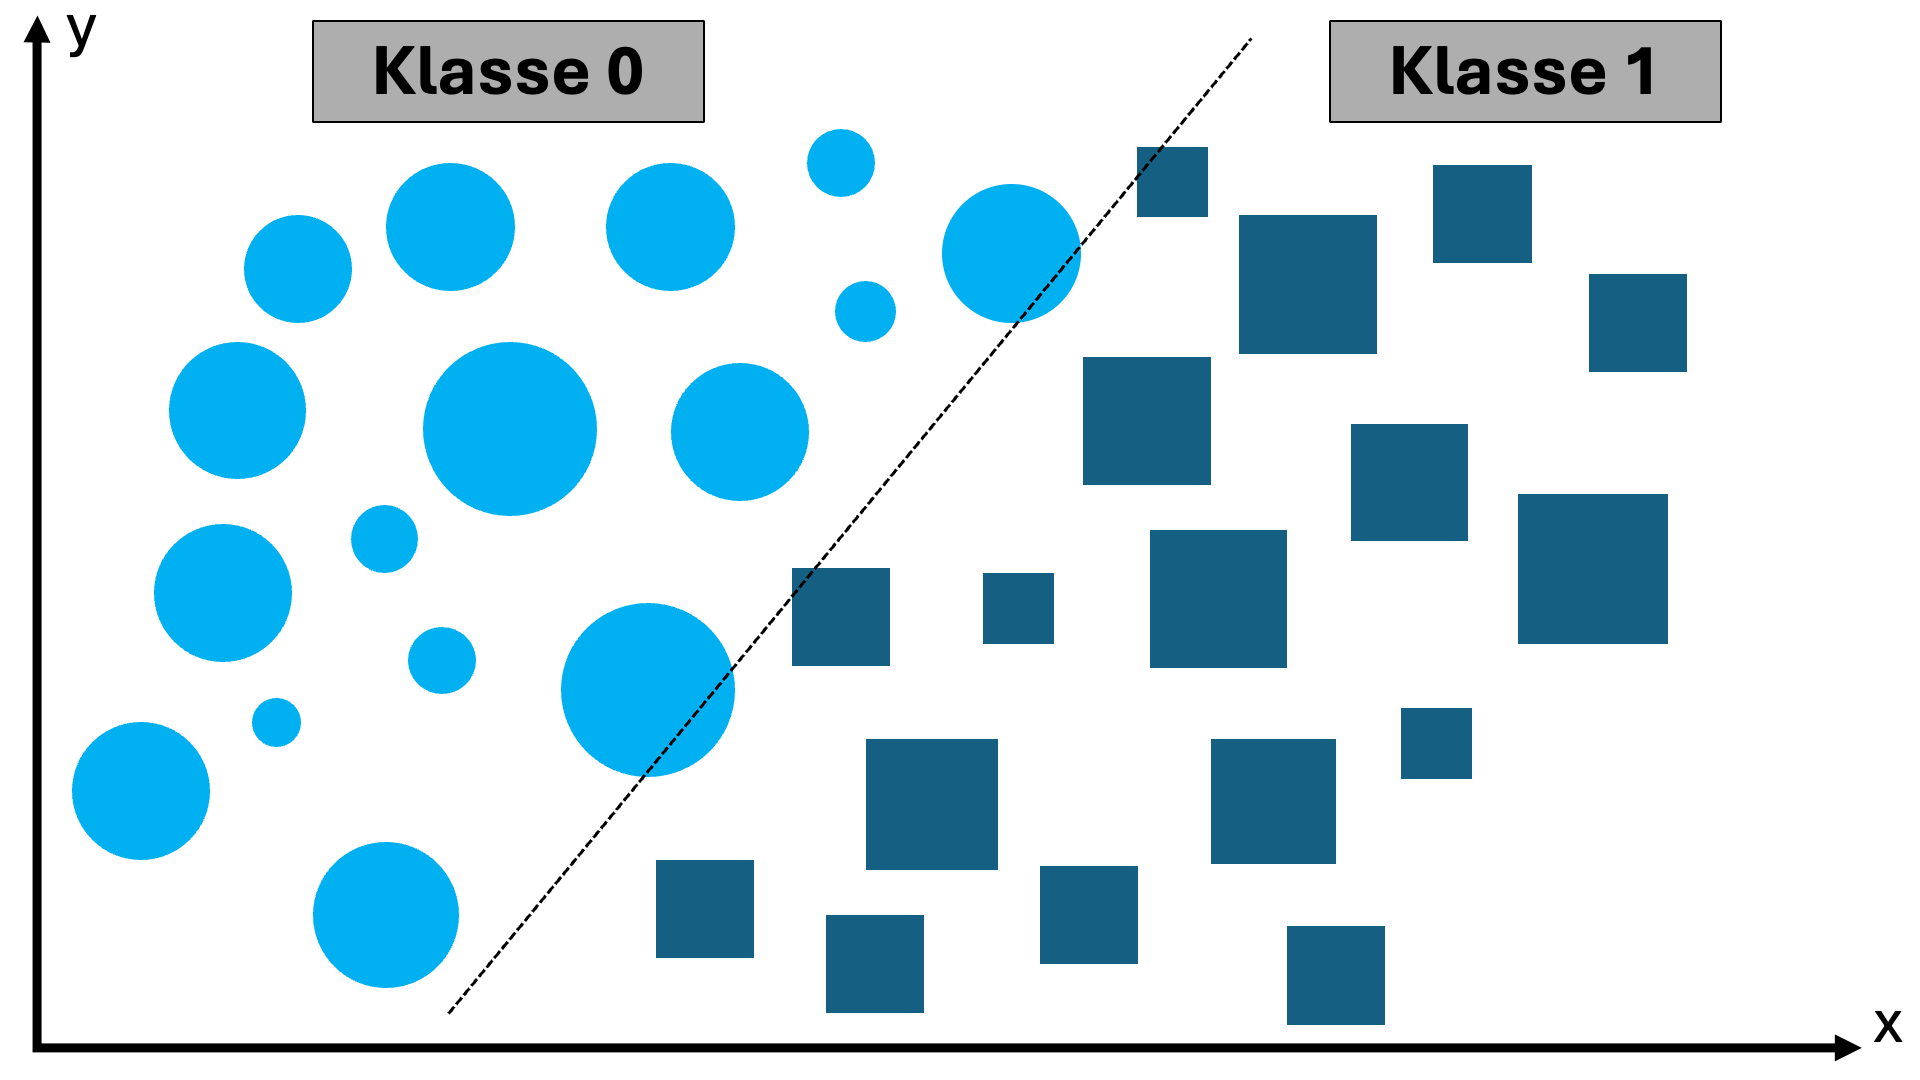
\includegraphics[width=\columnwidth]{binaere_klassifikation.png}}
    \caption{Darstellung der Programmarchitektur in Form eines Blockschaltbildes}
    \label{fig:bin_class}
\end{figure}

\subsection{Computer Vision}
\label{sec:computer_vision} 
Maschinelles Lernen stellt den Zusammenhang zwischen Eingangs- und Ausgabedaten her. Die wichtigsten Methoden sind überwachtes, unüberwachtes und Verstärkungslernen. In dieser Arbeit wurde überwachtes Lernen genutzt, bei dem ein Algorithmus mit gelabelten Daten trainiert wird. Neuronale Netze bestehen aus Eingabe-, versteckten und Ausgabeschichten. Convolutional Neural Networks (CNNs) sind besonders für Bildverarbeitung geeignet, da sie Bildmerkmale durch spezielle Faltungsebenen extrahieren.

Beim überwachten Lernen gibt es zwei Hauptmodelle: Klassifikation und Regression. Klassifikation teilt Daten in Gruppen ein, während Regression Zusammenhänge beschreibt. Die binäre Klassifikation unterscheidet zwei Klassen, dargestellt in Abbildung \ref{fig:bin_class}. Eine Entscheidungsgrenze trennt beide Klassen. In dieser Arbeit wird binäre Klassifikation verwendet, um das Geschlecht auf einem Bild zu erkennen.

Neben dem Training eigener Modelle können auch vortrainierte Modelle von Plattformen wie TensorFlow oder PyTorch geladen und feinabgestimmt werden.


\section{Datensatz} 
\label{sec:dataset}
In diesem Kapitel wird der verwendete Datensatz sowie die damit einhergehenden Herausforderungen beschrieben.

\subsection{Allgemeine Beschreibung des Datensatzes}
\label{sec:dataset_description}
Der Datensatz besteht aus ca. 2000 Bildern unterschiedlicher Qualität und Perspektive, die als JPEG-Dateien vorliegen. Zu jedem Bild existiert eine zugehörige Segmentierungsmaske im PNG-Format, welche Segmentierung beinhaltet. Zusätzlich enthält der Datensatz eine \texttt{tags.json}-Datei, die für jedes Bild das Geschlecht der abgebildeten Person zuordnet. Die Geschlechterverteilung innerhalb des Datensatzes umfasst ca. 1200 Bilder von Männern und 800 Bilder von Frauen.

\subsection{Herausforderungen bei der Datenverarbeitung}  
Die Nutzung dieses Datensatzes bringt mehrere Herausforderungen mit sich. Die variierende Bildqualität und unterschiedlichen Perspektiven könnten die Konsistenz der Segmentierung beeinträchtigen und die Generalisierbarkeit von Modellen erschweren. Zudem besteht eine Ungleichverteilung der Geschlechter mit 1200 Bildern von Männern und 800 von Frauen, was zu Verzerrungen in geschlechtsspezifischen Analysen führen kann. Die Qualität und Konsistenz der Segmentierungsmasken ist ein weiterer kritischer Faktor, da ungenaue oder fehlerhafte Masken die Modellleistung negativ beeinflussen könnten. Auch die Labels in der tags.json-Datei könnten Ungenauigkeiten enthalten oder nicht-binäre Identitäten ausschließen, was die Anwendbarkeit in diversen Szenarien einschränkt. Darüber hinaus erfordert die Verarbeitung von 2000 Bildern und Masken erhebliche Rechenleistung und Speicherplatz. 

Schließlich könnten je nach Anwendung weitere Herausforderungen auftreten, etwa wenn die Segmentierungsqualität oder Perspektivenvielfalt die Leistung eines Erkennungsmodells beeinträchtigt. Diese Aspekte sollten bei der Vorverarbeitung und Modellentwicklung sorgfältig berücksichtigt werden, um Verzerrungen zu minimieren und robuste Ergebnisse zu erzielen.

\section{Implementierte Lösung}

\begin{figure}[H]
    \centerline{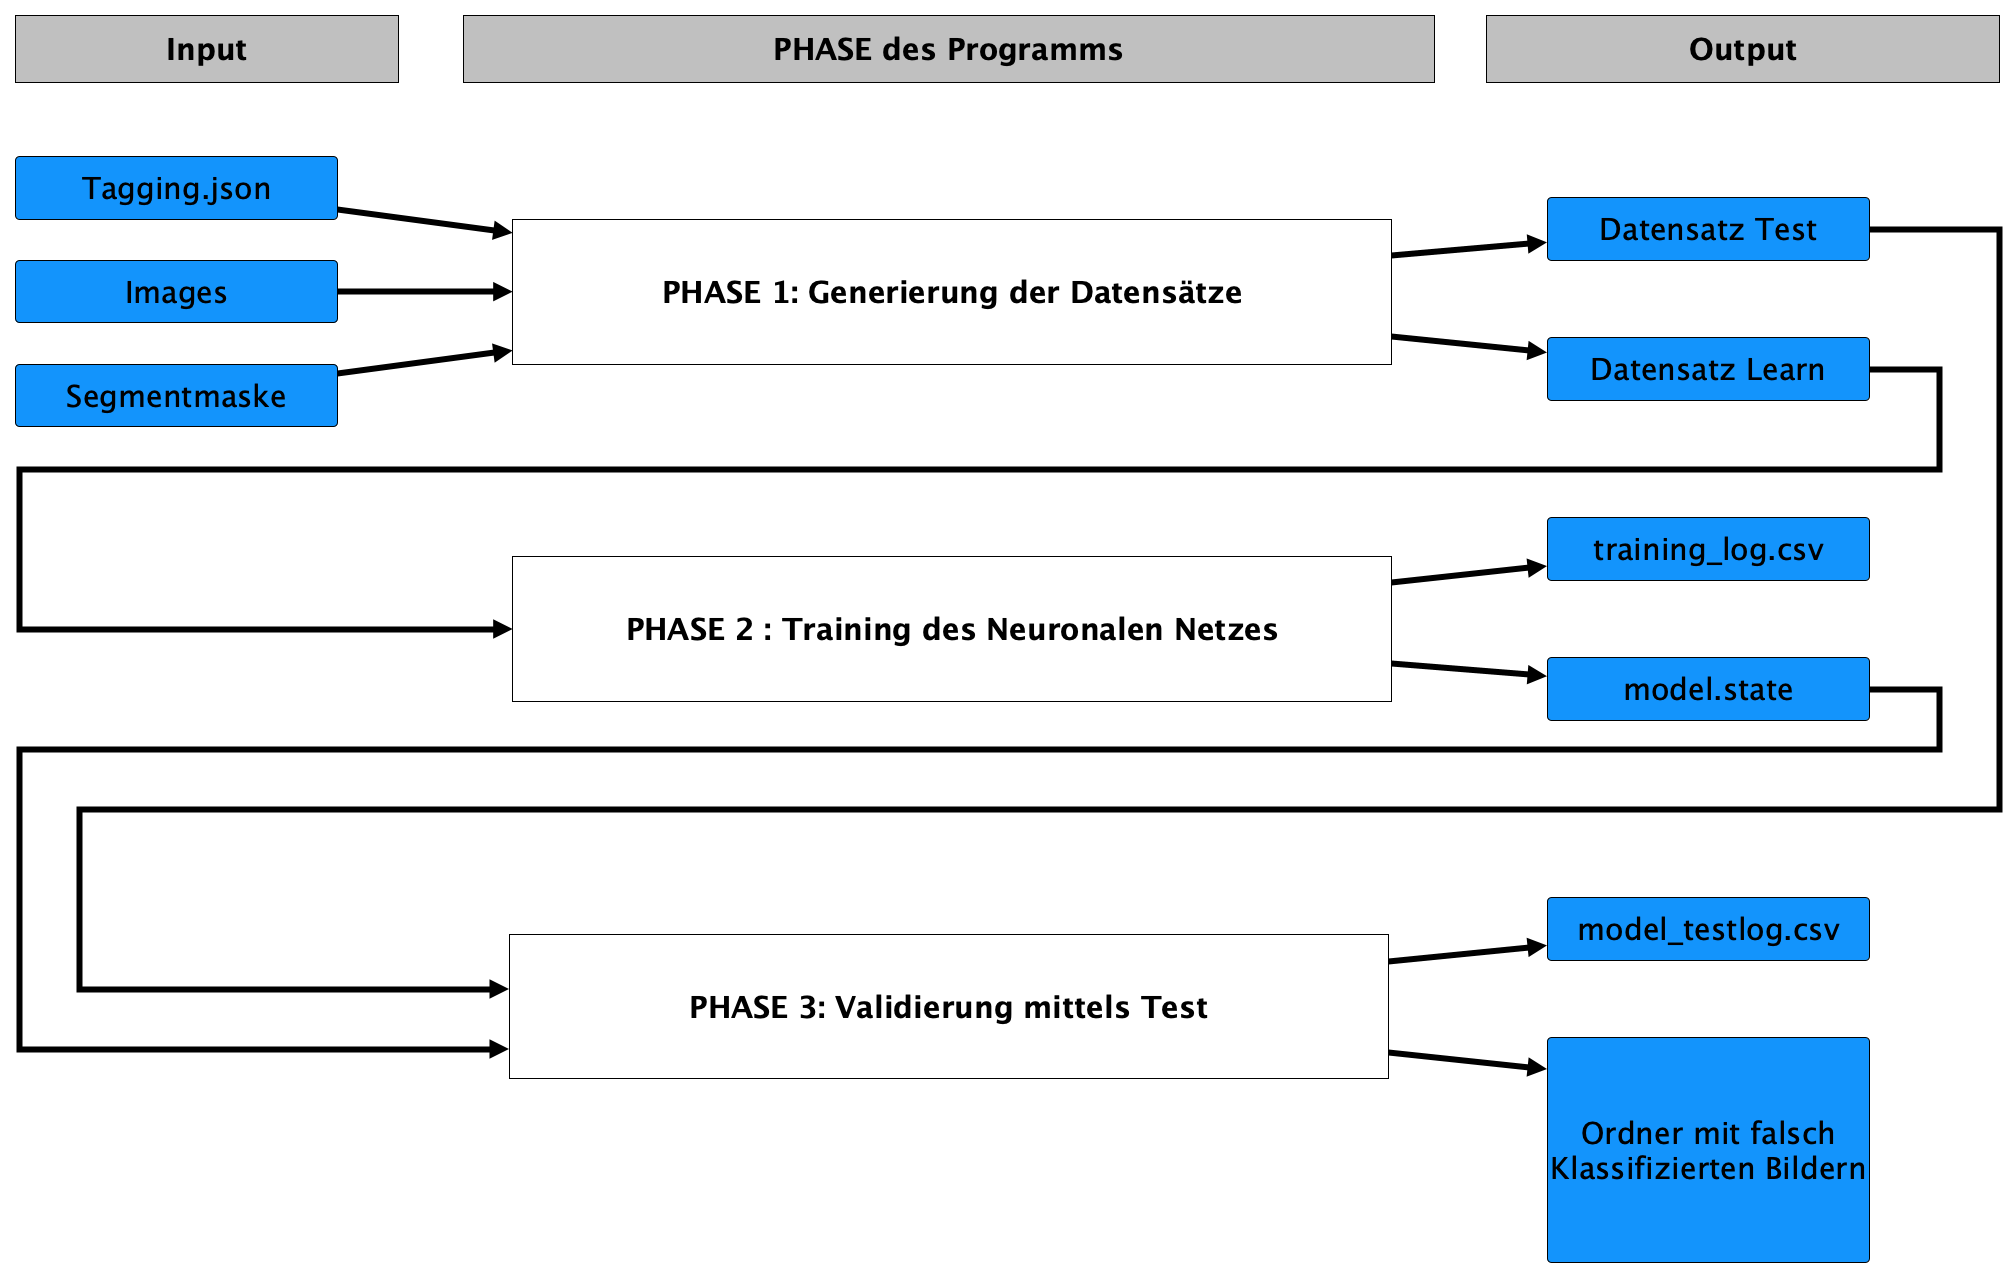
\includegraphics[width=\columnwidth]{Architektur.png}}
    \caption{Darstellung der Programmarchitektur in Form eines Blockschaltbildes}
    \label{fig:architecture}
\end{figure}

Die in Abbildung \ref{fig:architecture} dargetsellte Workflow beschreibt anschaulich die Implementierung des Lösungsvorschlags zu der Aufgabe Geschlechterklassifikation mit dem in Kapitel \ref{sec:dataset} beschriebenen Datensatz.
Im Folgenden wird eine genauere Beschreibung des Lösungsvorgangs gegeben.

\subsection{Generierung der Daten}
In der Datei \texttt{data\_generation.py} wird der in Kapitel \ref{sec:dataset_description} beschriebene Datensatz eingelesen und die Bilder mittels der Segmentierungsmasken verarbeitet. Hierbei geschieht die Verarbeitung wie Folgt. Den Bildern wird eine zusätzliche Farbebene (Alpha-Kanal) beigefügt, sowie die abgebildeten Personen freigestellt. Das resultierende Bild wird mittels einer affinen Transformation in eine einheitliche Position und Ausrichtung gebracht. Hierzu werden die Schwerpunkte der Konturen von Augen und Mund extrahiert und für die Berechnung der Transformationsmatrix bereitgestellt. Anschließend werden die Bilder in einem neuen Verzeichnis gespeichert, um sie für das Training und die Validierung des Modells zu verwenden.


\subsection{Training des Modells}
\label{sec:training}
Das Trainieren des Neuronalen Netzwerks geschieht in der Datei \texttt{classification.py}. Hierbei wird das Modell mit dem generierten Datensatz in mehreren Epochen trainiert. Die Trainingsdaten werden in Batches geladen und dem Modell übergeben. Nach jeder Epoche wird das Modell anhand eines Validierungsdatensatzes evaluiert, um die Genauigkeit der Klassifikation zu überprüfen. Das Training erfolgt iterativ, wobei die Gewichte des Modells angepasst werden, um die Klassifikationsgenauigkeit zu maximieren. Nach Abschluss des Trainings wird das Modell gespeichert und für die spätere Verwendung bereitgestellt. Die Während des Trainierens angewendeten Konzepte Data Augmentation und Early Stopping vermindern das Risiko von Overfitting und verbessern die Generalisierbarkeit des Modells.

Overfitting beschreibt die Situation, dass das Modell sich an nicht wesentliche Merkmale der Eingangsdaten anpasst. Vereinfacht erklärt: es lernt die Testdaten auswendig und kann dann nicht mehr auf wesentliche Merkmale Klassifizieren.

Data Augmentation beschreibt die Veränderung des Datensatzes, sodass der Datensatz größer wirk als er ist. 
Early Stopping beschreibt das Abbrechen des Trainings, wenn die Genauigkeit des Modells auf den Validierungsdaten nicht mehr steigt.


\subsection{Test des Modells}
Das Trainierte Modell wird in der \texttt{classification.py}-Datei getestet. Hierbei wird dem Modell batchweise der Testdatensatz übermittelt, welcher sich von dem Traingsdatensatz unterscheidet, übermittelt Die Klassifikationsergebnisse werden mit den tatsächlichen Labels verglichen, um die Genauigkeit des Modells zu bestimmen. Das Ergebnis wird in Form einer Erfolgsquote ausgegeben, die die Genauigkeit des Modells bei der Geschlechterklassifikation angibt. Zudem werden die falsch Klassifizierten Bilder in ein separates Verzeichnis gespeichert, um die Fehleranalyse zu erleichtern.

\subsection{Ausführung des Python Codes}

In diesem Kapitel wird beschrieben, wie der mit diesem Paper abgegebene Python Code ausgeführt werden kann.
Um die pipline der Datenverarbeitung mit Training der Daten und anschließendem Test des Modells durchzuführen, muss die Datei \texttt{classification.py} ausgeführt werden. Alle drei Dateien müssen im selben Verzeichnis liegen.

Hierfür muss sich ebenfalls im selben Verzeichnis wie die Datei \texttt{classification.py} ein Verzeichnis \texttt{Images} befinden, welches die Bilder und Masken enthält. Innerhalb dieses Verzeichnisses wird ebenfalls eine Datei \texttt{tags.json} benötigt, welche die Labels der Bilder enthält.

Der Ordner \texttt{Datensatz}, welcher später die Sortierten Bilder enthält, wird automatisch erstellt und in zwei Unterordner \texttt{Train} und \texttt{Test} unterteilt.

Falls es beim Ausführen des Codes zu Problemen kommt, kann es sein, dass die benötigten Bibliotheken nicht installiert sind. Diese können mit dem Befehl \texttt{pip install -r requirements.txt} installiert werden.

Damit nur ein Test des Modells durchgeführt wird können die Funktion \texttt{train\_model()} und \texttt{dg.preprocess()} in der Datei \texttt{classification.py} auskommentiert werden.


\section{Lösungsansätze im Vergleich}
In diesem Kapitel werden fünf Ansätze zur Implementierung des CNN vorgestellt. Insgesamt umfasst die Versuchsreihe 23 trainierte neuronale Netze unterschiedlicher einstellungen und Dimensionen.
Um der Anforderung an diese Dokumentation gerecht zu werden fällt die Wahl auf 5 Modelle die sowohl den Fortschritt, als auch den Wissensgewinn über die Zeit repräsentieren.

\begin{figure}[H]
    \centerline{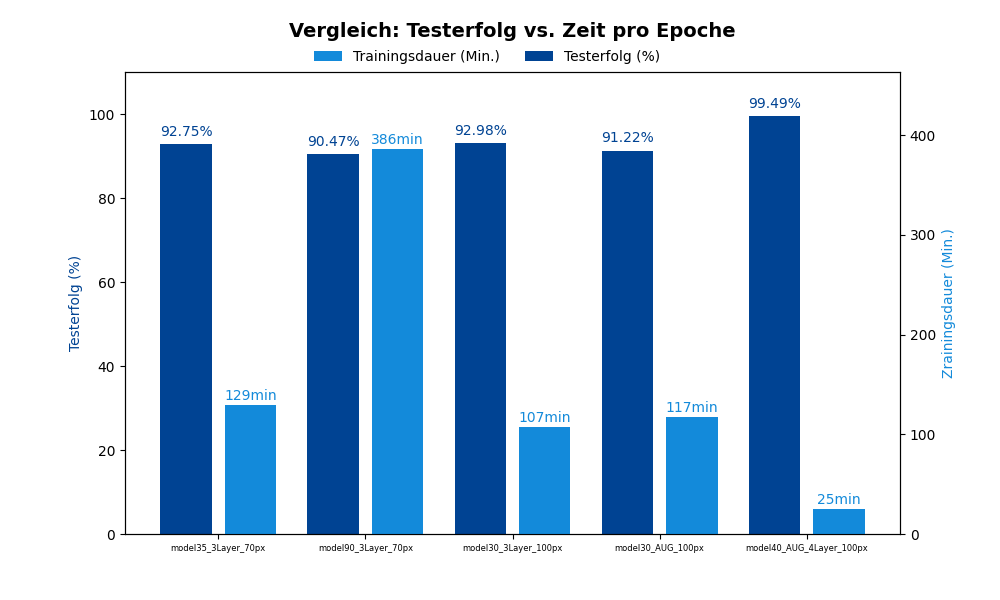
\includegraphics[width=\columnwidth]{Erfolg_Dauer.png}}
    \caption{Vergleichsdiagramm zwischen Erfolgsquote des jeweiligen Modells im Test gegenüber der Dauer einer Trainingsepoche.}
    \label{fig:compareGraph}
\end{figure}

\subsection{Ablauf der Optimierung}
\label{sec:optimization}
Als Grundlage für das Design des neuralen Netz dient ein im Labor verwendeter Python-Pytorch Code. Dieser Code ist in seinen Parametern ergänzt, um den verwendeten Bildgrößen und Bildkanälen gerecht zu werden. 

Mit dem ersten Prorgammentwurf entsteht das netz "Model35", welches zunächst den besten Wert im Test liefert. Dieses Modell ist mit drei Faltungsebenen und einer Reduktion auf 256*26*35 linearen Datenpunkten ausgestattet.
Es wurde für den Test in 35 Epochen trainiert und liefert $92,7\%$ Genauigkeit im Test (Siehe Abbildung: \ref{fig:compareGraph})

Der erste Ansatz der Optimierung ist die erhöhung der Trainingsepochen. Bei gleichbleibenden Modellparametern wird mit 90 Statt 35 Epochen Trainiert.
Dies hat maßgeblichen Einfluss auf die gesamtdauer, die mit 386min deutlich über den 129min des Vorängers liegt (Siehe Abbildung: \ref{fig:compareGraph}). Dies hat keinen positiven Effekt auf den Erfolg des Tests.

\begin{figure}[H]
    \centerline{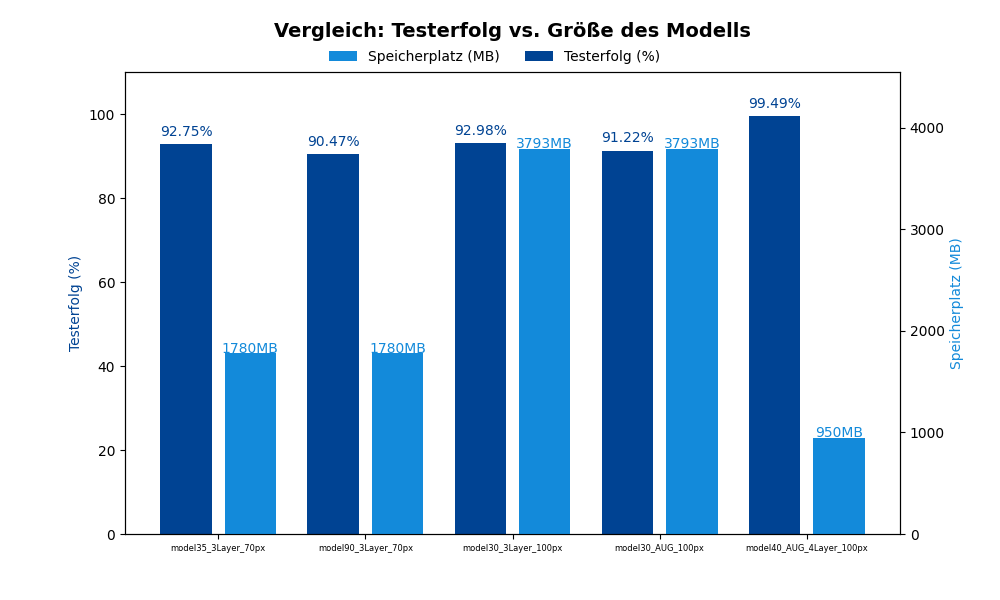
\includegraphics[width=\columnwidth]{Erfolg_Groesse.png}}
    \caption{Vergleichsdiagramm zwischen Erfolgsquote des jeweiligen Modells im Test gegenüber dem Verbrauchten Speicherplatz.}
    \label{fig:compareSize}
\end{figure}

Der nächste Optimierungsansatz besteht in der erhöhung der Bildauflösung. Die zuvor festgelegten 70px für den Augenabstand werden auf 100px erhöht, was eine Auflösungserhöhung von 210x280 auf 300x400 bedeutet.
Der Augenabstand ist die maßgebliche Größe, um die Segmentierung und Transformation des Bildes durchzuführen.

Diese Erhöhung sorgt für eine Steigerung der Modellkomplexität, da die zuvor verwendeten 256*26*35 Datenpunkte nun auf 256*37*50 erhöht wurden. 
Durch die zusätzlichen Informationen ist eine Stegerung des Erfolges um $0,2\%$ möglich. Durch die Erhöhung der Komplexität und damit auch der Kapazität des Modells auf fast das Doppelte (Siehe Abbildung \ref{fig:compareSize}), ist eine Betrachtung der Overfitting-Problematik unabdingbar.

Um dieser Problematik entgegen zu wirken wurden die im Kapitel \ref{sec:training} erklärten Konzepte Data Augmentation und Early Stopping in den Programmcode implementiert.

Das Modell (model30\_AUG\_3Layer\_100px) erzielt trotz Augmentation keine Verbesserung des Traingserfolges, sondern verschlechtert diesen mit $91,22\%$. 
Ohne den Augmentation Ansatz zu verwerfen ist die nächste Optimierung die Ergänzung einer weiteren Faltungsebene. 
Dies Reduziert die Linearen Parameter und damit auch die Komplexität des Modells, was sich postiv auf die Traningsdauer auswirkt. 
In einem ersten Test konnte dieses Letzte Modell (model40\_AUG\_3Layer\_100px\_ES) zunächst $94\%$ und in einem zweiten Test $99\%$ erzielen.

\subsection{Diskussion der Lösungsansätze}
Alle drei Lösungsansätze bieten solide Ergebnisse für das Klassifikationsproblem. Keines der vorgestellten Modelle liefert Ergebnisse schlechter als $80\%$ Hinsichtlich der Komplexität und der benötigten Rechenressourcen zeigt sich jedoch, dass das Modell mit Data Augmentation und einer zusätzlichen Faltungsebene (model40\_AUG\_3Layer\_100px\_ES) die besten Resultate erzielt. Es kombiniert eine hohe Genauigkeit mit einer moderaten Trainingsdauer und Speicherplatzanforderung, was es zu einer effizienten und effektiven Lösung für die Geschlechterklassifikation macht (Abbildung \ref{fig:compareGraph} und Abbildung \ref{fig:compareSize}).

Die anderen Modelle liefern hinsichtlich des Erfolges ebenfalls solide Resultate. 
Unter Berücksichtigung der zeitlichen Komponente des Optimierungsfortschrittes hinsichtlich des Codeaufbaus der fünf Modelle sind die anfangs erreichten $92,75\%$ ebenfalls nicht zu vernachlässigen. Hier wurden $7\%$ weniger erzielt als beim besten Modell, allerdings mit fünf Tagen weniger Arbeitsaufwand für die Codeoptimierung. 

Die dazwischen getesteten Modelle stellen verschiedene Optimierungsversuche dar, die im Laufe der Entwicklung durchgeführt wurden. Die Beschreibung dieser Optimierungen und deren Auswirkungen auf die Modellleistung sind im letzten Kapitel (Kapitel: \ref{sec:optimization}) dokumentiert.

\section{Fazit}
\label{sec:conclusion}
In dieser Arbeit wurde die Verarbeitung und Klassifikation von Gesichtsaufnahmen zur Geschlechterklassifikation mittels neuronaler Netze untersucht. Der Wissensgewinn über die Zeit war erheblich, da verschiedene Modelle und Optimierungsansätze getestet und evaluiert wurden. Beginnend mit einem einfachen Modell, das bereits eine solide Genauigkeit erzielte, wurden durch schrittweise Optimierungen wie die Erhöhung der Bildauflösung, die Implementierung von Data Augmentation und Early Stopping sowie die Anpassung der Netzwerkarchitektur signifikante Verbesserungen erreicht.

Die besten Ergebnisse wurden mit einem Modell erzielt, das Data Augmentation und eine zusätzliche Faltungsebene nutzte, was die Genauigkeit auf bis zu $99\%$ steigerte. Dies zeigt, dass durch gezielte Optimierungen und Anpassungen erhebliche Leistungssteigerungen möglich sind.

Als Ausblick soll nicht unerwähnt bleiben, dass weitere Verbesserungen durch den Einsatz fortschrittlicherer Aktivierungsfunktionen wie Sigmoid möglich gewesen wären. Diese könnten die Klassifikationsgenauigkeit weiter erhöhen, indem sie nichtlineare Beziehungen in den Daten besser modellieren. Zukünftige Arbeiten könnten sich darauf konzentrieren, diese und andere fortschrittliche Techniken zu integrieren, um die Modellleistung weiter zu optimieren.

Insgesamt zeigt diese Arbeit, dass durch iterative Optimierung und den Einsatz moderner Techniken in der Bildverarbeitung und im maschinellen Lernen robuste und leistungsfähige Modelle zur Geschlechterklassifikation entwickelt werden können.






\appendices

% \section*{Appendix und die Nutzung von ergänzenden Dateien}

\section*{Danksagung}

\end{document}
